% Chapter 2 - Background

\glsresetall % reset the glossary to expand acronyms again
\chapter[Literature Review]{Literature Review}\label{ch:LitReview}
\index{Literature Review}

% Literature Review
This chapter assesses existing medical imaging denoising techniques, specifically focusing on their applicability to LODOX\textsuperscript{\textregistered} Statscan\textsuperscript{\textregistered} images.  It starts with a review of X-ray imaging theory, establishing a foundation to understand the unique challenges posed by LODOX\textsuperscript{\textregistered} Statscan\textsuperscript{\textregistered} system.  After that, it delves into a discussion of the specific image artifacts associated with this technology.  Finally, denoising algorithms used in Medical imaging are critically evaluated, assessing their suitability to LODOX\textsuperscript{\textregistered} Statscan\textsuperscript{\textregistered} images.


\section{X-ray Imaging Fundamentals}
\label{ch:LitReview:X-ray Imaging Fundamentals}
This section summarises the theoretical framework and principles of X-ray imaging. Understanding the core principles of X-ray imaging is fundamental to improving the X-ray imaging quality through denoising, particularly in the context of low-dose systems like LODOX\textsuperscript{\textregistered} Statscan\textsuperscript{\textregistered}. The following subsections will look into mechanisms of X-ray production, X-ray detection and image formation.

The fundamental X-ray imaging theory, including X-ray generation, interaction with matter, and image formation, is extensively covered in \cite{haidekker_introduction_2013},\cite{haidekker_x-ray_2013},\cite{haidekker_trends_2013}, providing a solid foundation for the subsequent discussion.



\subsection{X-ray Production}
\label{ch:LitReview:X-ray Production}
X-rays are generated in an X-ray tube by accelerating high kinetic energy electrons from the cathode across the electrostatic field in the vacuum towards the anode, striking the anode emitting X-rays. 

X-ray emission is primarily controlled by the anode voltage, which dictates the maximum energy of the X-ray photons, and the tube current, which determines the photon flux. These parameters directly influence image quality by affecting the photon count detected by the X-ray detectors. Additionally, the focal spot size of the X-ray tube plays a crucial role in image resolution as it determines the size of the X-ray beam. For instance, when the image details to be captured are smaller than the X-ray beam diameter, geometric blur is observed, which degrades image quality.

X-ray production is only one part of the imaging process; once generated, these Xrays must travel through various tissues, where their attenuation plays a critical role in the resulting image quality.






\subsection{X-ray Attenuation}
\label{ch:LitReview:X-ray Attenuation}
X-ray attenuation across various bodies is what brings about X-ray contrast. X-ray attenuation occurs when the X-ray photons collide with other atoms and get deflected from their path whilst losing some energy. The major forms of X-ray attenuation are Rayleigh Scattering, Compton Scattering, Photoelectric effect and pair production. These are summarised in the Table  \ref{XrayAttenuation} below:

\begin{center}
\small
\setlength{\arrayrulewidth}{1mm} % Thicker outer border
\setlength{\tabcolsep}{6pt} % Increase cell padding
\renewcommand{\arraystretch}{1.5} % Increase row height for readability



\begin{longtable}{ p{0.25\columnwidth}  p{0.25\columnwidth}  p{0.4\columnwidth} }

	%\hline
	\rowcolor[HTML]{D3D3D3}
	\textbf{Interaction} & \textbf{Photon Energy Range} & \textbf{Significance in Medical Imaging} \\
	%\hline
	\rowcolor[HTML]{FFFFFF} 
	Rayleigh Scattering & Low Photon Energies & Negligible Above 50 keV thus negligible influence on image quality \\
	%\hline
	\rowcolor[HTML]{F3F3F3} 
	Compton Scattering & All Photon Energies & Characteristic radiation leading to scattering that causes haze in the images. \\
	%\hline
	\rowcolor[HTML]{FFFFFF} 
	Photoelectric Effect & 50-70 keV & Crucial for X-ray contrast, especially at lower energies \\
	%\hline
	\rowcolor[HTML]{F3F3F3} 
	Pair Production & Above 1.02 MeV & Limited relevance in medical imaging as rarely seen in practice \\
	%\hline
	
	\caption{Summary of Photon Interaction Mechanisms and Their Significance in Medical Imaging.}
	\label{XrayAttenuation}

\end{longtable}
\end{center}

 In  LODOX\textsuperscript{\textregistered} Statscan\textsuperscript{\textregistered}, scattering is not an issue due to the unique detector architecture that reduces scattering by up to 95\%\cite{amirlak_novel_2009}. As X-rays are attenuated as they pass through different tissues, this varying absorption information must be recorded to generate X-ray images. The following subsection will look into the X-ray detection and image formation mechanism and how it affects the image quality.

\begin{comment}
    \begin{table}[h!]
\centering

\begin{tabular}{| p{0.25\columnwidth} | p{0.25\columnwidth} | p{0.45\columnwidth} |}
\hline

\textbf{Interaction} & \textbf{Photon Energy Range} & \textbf{Significance in Medical Imaging} \\
\hline
Rayleigh Scattering & Low Photon Energies & Negligible Above 50 keV thus negligible influence on image quality \\
\hline
Compton Scattering & All Photon Energies & Characteristic radiation leading to scattering that causes haze in the images. \\
\hline
Photoelectric Effect & 50-70 keV & Crucial for X-ray contrast, especially at lower energies \\
\hline
Pair Production & Above 1.02 MeV & Limited relevance in medical imaging as rarely seen in practice \\
\hline

\end{tabular}
\caption{Summary of Photon Interaction Mechanisms and Their Significance in Medical Imaging.}
\label{XrayAttenuation}

\end{table}
\end{comment}





\subsection{X-ray Detection and Image Formation}
\label{ch:LitReview:X-ray Detection and Image Formation}
This subsection delves into how X-ray photons are converted and detected for imaging. X-ray intensity is primarily measured using photographic films and digital detectors, necessitating conversion to another energy form, usually visible light or \gls{UV}  photons. Digital detectors are predominantly used today, as older photographic films and fluoroscope detectors were phased out due to their very low quantum efficiency and sensitivity. 

During the conversion process, these digital detectors introduce various noise components, including electronic noise and quantum noise due to the use of \gls{ASIC}. In addition, converting X-ray photons into electrical signals can introduce image artifacts such as detector blur. Detector blur occurs due to the conversion layer, which typically emits visible light in all directions. A thick conversion layer increases the likelihood of cross-talk between neighbouring pixels, while a thinner conversion layer reduces this effect and lowers quantum efficiency. Keeping the conversion layer close to the detector element can help mitigate detector blur.

Motion blur is another significant factor impacting image quality, which arises when the patient moves during exposure due to breathing. High detector sensitivity and a high photon flux from the X-ray source can allow for shorter exposure times, which reduces the likelihood of motion blur affecting the final image.




\section{Noise in X-ray imaging}
\label{ch:LitReview:Noise in X-ray imaging}
This section will examine the various types of noise inherent in X-ray imaging, specifically low-dose X-ray imaging systems such as the LODOX\textsuperscript{\textregistered} Statscan\textsuperscript{\textregistered}. It then proceeds to discuss the sources of these noises in the LODOX\textsuperscript{\textregistered} Statscan\textsuperscript{\textregistered} and concludes with an analysis of the impact of the noise on image quality and diagnosis. 


\subsection{Types of Noise in X-ray Imaging}
\label{ch:LitReview:Types of Noise in X-ray Imaging}
Noise is defined as random unwanted stochastic fluctuations and variations in brightness and colour information in an image \cite{veldkamp_dose_2009}, \cite{lahmiri_iterative_2017}. In X-ray, there are various noise types, each with a different statistical model arising from multiple sources such as the detectors' inherent properties, X-ray source, inspected objects and controller circuits \cite{seibert_tradeoffs_2004}, \cite{noauthor_noise_nodate}. The primary noise present in X-rays is Quantum noise. Other prominent noise types include Electronic and Anatomical noise. These three noise types are discussed below:


\textbf{Quantum Noise}\\
Studies show that quantum noise is predominant in \gls{PCD} \cite{noauthor_noise_nodate}, \cite{huda_radiographic_2015}. Given that \gls{PCD} are the detectors currently being used in the LODOX\textsuperscript{\textregistered} Statscan\textsuperscript{\textregistered} it is paramount to understand quantum noise. Quantum noise results primarily from X-ray photon detection and conversion \cite{kim_measurements_2024}, \cite{seibert_tradeoffs_2004}. It is produced due to the random accumulation and distribution of the X-ray photons on the detectors’ surface \cite{noauthor_noise_nodate}, \cite{veldkamp_dose_2009}, \cite{manson_image_2019}, \cite{chandra_analysis_2020}, \cite{juneja_denoising_2024}. This is shown in the Figure \ref{PoissonGen} below:
\begin{figure}[h!]
    \centering
    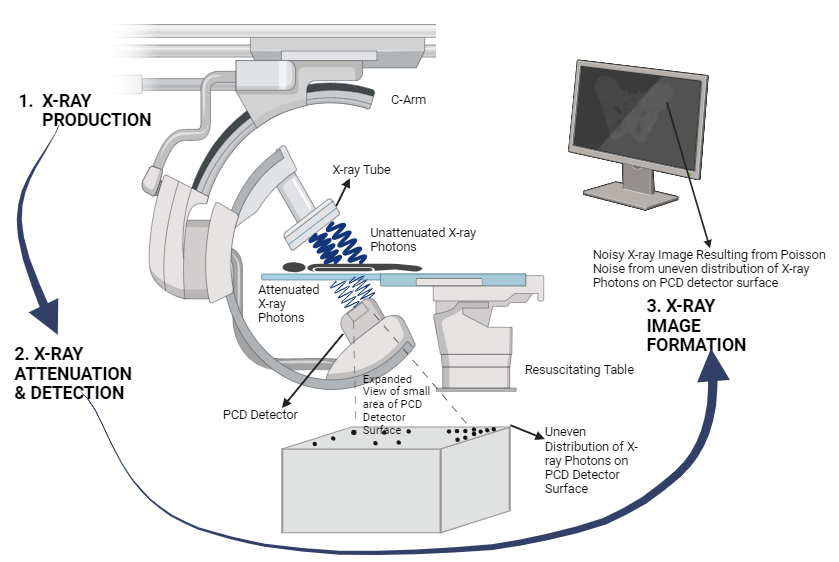
\includegraphics[width=0.5\linewidth]{3_Chapters//2_Chapter_LiteratureReview//Figures/PoissonNoise Prodcution.png}
    \caption{Diagram illustrating the generation of quantum noise in X-ray imaging due to the uneven distribution of X-ray photons on the PCD detector surface, resulting in a noisy image output. Created with \href{https://www.biorender.com}{BioRender.com}  }
    \label{PoissonGen}
\end{figure}

Due to the wide spectrum energy of X-ray photons and the randomness mentioned above, quantum noise is modelled using the Poison distribution as shown below:
\begin{equation}
P(x) = e^{-\lambda t} \frac{(\lambda t)^k}{x!}
\label{eq:poisson}
\end{equation}
Where:
\begin{table}[h!]
    %\centering
    \begin{tabular}{cc}
         P(x):& probability of distribution of photons \\
         $\lambda$:& Expected number of photons \\
         X :& measured number of photons\\
         t :& given time interval\\
    \end{tabular}
    
\end{table}

Equation \ref{eq:poisson}  depicts the signal-dependent nature of quantum noise, indicating it is not an additive noise like \gls{AWGN} as shown in studies  \cite{khan_new_2016}, \cite{thanh_review_2019}, \cite{chandra_analysis_2020}. Since quantum noise follows Poisson distribution, the expected photon count (E(x)) is equal to the variance of the photon count(var(x)) over the given time interval in Equation \ref{eq:poisson}. Thus quantum noise is proportional to the square root of the number of photons captured by the detector \cite{chandra_analysis_2020} and the square root of radiation exposure \cite{huda_radiographic_2015} as shown in equations \ref{eq:numphotons} and \ref{eq:radexposure} below:

\begin{equation}
\begin{aligned}
    E[x] &= \text{var}[x] = \lambda t \\
    \text{std}[x] &= \sqrt{\lambda t}
\end{aligned}
\label{eq:numphotons}
\end{equation}


\begin{equation}
    \sqrt{exposure level}
    \label{eq:radexposure}
\end{equation}

From the above, it can be deduced that by increasing the X-ray radiation and exposure time, quantum noise can be reduced \cite{chandra_analysis_2020}; however, this is not a suitable method in the LODOX\textsuperscript{\textregistered} Statscan\textsuperscript{\textregistered} system as it is inherently a low-dose X-ray system. 


\textbf{Electronic Noise} \\
Electronic noise typically arises from random signals caused by thermal fluctuations in interconnected electronics \cite{gravel_method_2004}, amplifier noise \cite{goyal_noise_2018}, and imperfections in detectors, such as thickness variations, scratches, and dust on the detector substrate \cite{seibert_tradeoffs_2004}. Additionally, voltage variations over the long signal distances in large detectors contribute to this noise \cite{kim_measurements_2024}. This type of noise is prevalent in \gls{CCD} \cite{gravel_method_2004} and is most pronounced at lower X-ray energy levels \cite{veldkamp_dose_2009}.

Electronic noise is modelled using the Gaussian distribution as shown in Equation \ref{eq:gaussian} as it emanates from random signals \cite{juneja_denoising_2024}:

\begin{equation}
G(x) = \left( \frac{1}{\sigma \sqrt{2\pi}} \right) e^{-\frac{(x - \mu)^2}{2\sigma^2}}
\label{eq:gaussian}
\end{equation}
Where:
\begin{table}[h!]
    %\centering
    \begin{tabular}{cc}
         $\sigma$:& represents the standard deviation \\
         X :& represents the value of the pixel \\
         $\mu$ :& represents the mean \\
    \end{tabular}
    
\end{table}

Since the LODOX\textsuperscript{\textregistered} Statscan\textsuperscript{\textregistered} now uses \gls{PCD} instead of \gls{CCD}, the impact of electronic noise is significantly reduced, with the primary source being the low X-ray doses used.


\textbf{Anatomical Noise} \\
Anatomical noise is caused by the projection of the 3D object of interest to a 2D plane, resulting in the overlapping of anatomical objects in the region of interest in the image \cite{veldkamp_dose_2009}, \cite{seibert_tradeoffs_2004}. This overlap leads to local and global camouflaging that obstructs critical parts of the image \cite{seibert_tradeoffs_2004}
. Studies have shown that anatomical noise is particularly prevalent at very low X-ray energy levels \cite{veldkamp_dose_2009}. Notably, anatomical noise is one of the most challenging to correct and affects all X-ray systems \cite{seibert_tradeoffs_2004}.

\begin{comment}
In addition to the three primary noise sources in X-ray systems discussed above, Table \ref{tab:secnoisesources} summarises less impactful secondary noise sources that primarily affect the Contrast to Noise Ratio.


\begin{table}[h!]
\tiny
\centering

\begin{tabular}{|  p{0.25\columnwidth} |  p{0.75\columnwidth} |}
\hline
\textbf{Secondary Noise Source} & \textbf{Description} \\
\hline
\textbf{Swank Noise} & Results from the variation in light output as a function of absorption depth in a scintillator, adding to the overall noise. \\
\hline
\textbf{Spatial Sampling and Quantization Errors} & Occur during the conversion of a continuous analogue signal into a discrete digital signal. \\
\hline
\textbf{Scatter} & If an antiscatter grid is used, grid cutoff or grid lines can inject unwanted noise into the image. \\
\hline
\textbf{Errors in Flat Fielding Correction} & Flat fielding is used to reduce noise caused by stationary detector non-uniformities. It works by acquiring a uniformly exposed, low-noise image (or series of images) to identify and correct variations by applying a normalized and inverted correction image. \\
\hline
\textbf{Aliasing} & A distortion that occurs when a high-frequency signal is undersampled, leading to artifacts in the image. \\
\hline

\end{tabular}
\caption{Table: Secondary Noise Sources Affecting Contrast to Noise Ratio in X-ray Systems}
\label{tab:secnoisesources}
\end{table}

\end{comment}

 

\subsection{Impact of Noise on Image Quality and Diagnosis}
\label{ch:LitReviewImpact of Noise on Image Quality and Diagnosis}

Noise in X-ray systems significantly impacts image quality, particularly at low doses \cite{veldkamp_dose_2009}. It can introduce obstructions that render images non-diagnostic \cite{manson_image_2019}. Additionally, it can introduce artifacts that hinder the acquisition of quality images, potentially leading to false diagnoses\cite{goyal_noise_2018}. Moreover, degradation in image quality makes visual interpretation difficult\cite{warner_understanding_2020}, \cite{lahmiri_iterative_2017}
, complicating diagnostics for medical professionals \cite{khan_new_2016}. Finally, the corruption of X-ray images due to noise further impairs diagnostic accuracy\cite{chandra_analysis_2020},\cite{umadevi_improved_2011}
,\cite{dong_x-ray_2020} ultimately hindering effective clinical decision-making.


\section{Denoising}
From section \ref{ch:LitReviewImpact of Noise on Image Quality and Diagnosis}, it has been established that noise degrades the image quality, thus making denoising a critical part of the pre-processing chain. The primary objective of denoising is to effectively suppress noise while preserving the image integrity \cite{juneja_denoising_2024},  \cite{lahmiri_iterative_2017}, \cite{kumar_noise_2017}. Broadly, there are three X-ray denoising methods, as shown below:

\begin{enumerate}
    \item \textbf{Use of customised hardware:} Done through incorporating hardware filters such as Aluminium filters in the X-ray machines to help reduce noise \cite{lee_impact_2022}.
    \item \textbf{Increase in X-ray dose:} An increase in the X-ray dose used significantly reduces the noise in the image. However, the dose is hindered by the Maximum Permissible Dose(MPD); thus, the dose cannot be arbitrarily increased \cite{kirti_poisson_2017}.
    \item \textbf{Digital Denoising Algorithms:} Involves using digital image processing algorithms to reduce the noise digitally.
\end{enumerate}

Digital denoising algorithms are widely used as they are not as expensive as hardware customisation and do not increase radiation risk to the patients as the increasing X-ray dose method, thus making it the most effective technique to consider for denoising LODOX\textsuperscript{\textregistered} Statscan\textsuperscript{\textregistered} images. 

The type of noise in the images significantly impacts the effectiveness of denoising algorithms, and studies caution against the assumption that all noise is \gls{AWGN} \cite{kirti_poisson_2017}. As highlighted in Section \ref{ch:LitReview:Types of Noise in X-ray Imaging}, quantum noise is the most common in X-ray images, especially in low-dose settings. Consequently, noise-independent denoising algorithms do not work well on X-ray images, making Poisson-based methods the preferred approach \cite{thanh_review_2019}, \cite{kipele_poisson_2023}. Studies have suggested two approaches to handle Poisson noise, as discussed below:

\begin{enumerate}
    \item \textbf{Poisson Direct Denoising methods}: Model the Poisson noise statistics, which are usually helpful when the images suffer from very high noise levels \cite{kirti_poisson_2017}, \cite{kipele_poisson_2023}.
    \item \textbf{Poisson \gls{VST} Denoising methods:} Involves transforming the Poisson noise to Gaussian noise because when the photon count is large enough, Poisson distribution approaches Gaussian, and the \gls{Anscombe transform} is used to stabilising the variance of the Poisson noise \cite{kipele_poisson_2023}.
\end{enumerate}

However, denoising X-ray images presents several critical challenges discussed below:

\begin{enumerate}
    \item \textbf{Maintaining flat regions:} Flat regions in the image must remain flat without introducing noise or artifacts \cite{juneja_denoising_2024}.
    \item \textbf{Preserving image boundaries:} Image boundaries must be retained without causing blurring \cite{juneja_denoising_2024}.
    \item \textbf{Protecting global contrast and textural features:} The global contrast should be preserved, and textural details should not be lost [19].
    \item \textbf{Avoiding new artifacts:} The denoising process should not generate any new artifacts in the image \cite{juneja_denoising_2024}, \cite{thanh_review_2019}.
\end{enumerate}
 
 
Over the years, various algorithms have been proposed to address these four challenges. These algorithms are generally classified into three broad categories: Classical Filters, Hybrid Filters and Deep learning methods \cite{juneja_denoising_2024}, \cite{kirti_poisson_2017}. The following section will analyse each category in detail, exploring their advantages, disadvantages, and suitability for handling Poisson noise in the LODOX\textsuperscript{\textregistered} Statscan\textsuperscript{\textregistered}.

\subsection{Classical Filters}
This subsection briefly discusses the classical \gls{DSP} filters implemented to combat noise in X-ray Images, broadly classified into spatial and transform filters as shown in Figure \ref{fig:classicflo} below.  Spatial filters are further categorised into linear and non-linear filters. Linear filters are easy to implement as they apply non-discriminate denoising to all the pixels without prior categorisation \cite{khan_new_2016} and thus are not good with signal-dependent noise leading to artifacts and blurring \cite{juneja_denoising_2024}, \cite{mandic_denoising_2018}. In contrast, non-linear filters first detect noisy pixels and then replace them selectively, making them more effective for denoising \cite{khan_new_2016}. Unlike spatial filters, transform domain filters operate by converting the image into an alternative representation, such as the Wavelet or Fourier domain, where denoising is performed, after which the image is transformed back to the spatial domain using an inverse transform.

\begin{figure}[h!]
	\centering
	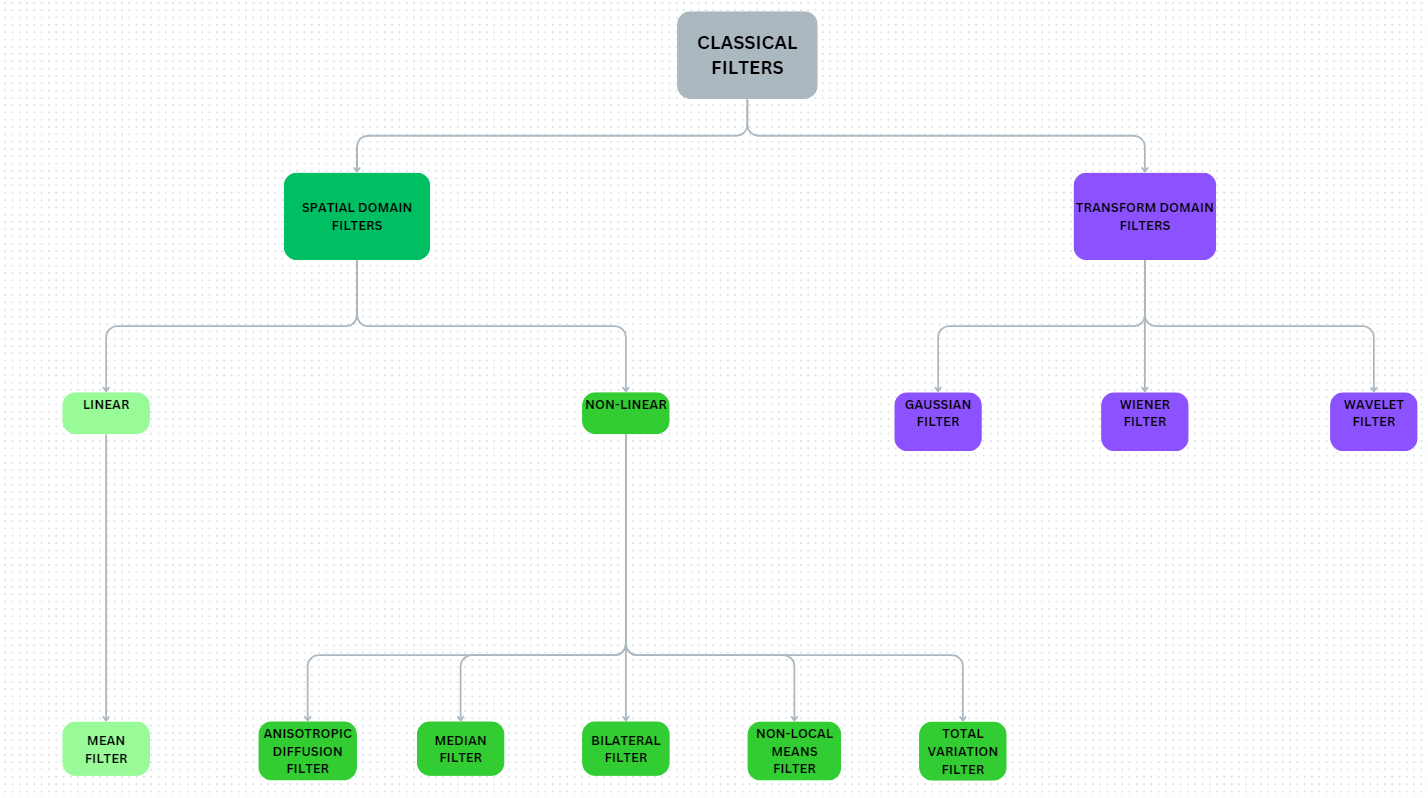
\includegraphics[width=0.9\linewidth]{3_Chapters//2_Chapter_LiteratureReview//Figures/ClassicalFlowchart.png}
	\caption{Flowchart summarising the classical filters used in X-ray image denoising}
	\label{fig:classicflo}
\end{figure}


Studies have shown that most classical filters struggle to handle photon-limited images. For instance, \gls{ADF} performance on photon-limited noise degrades with increasing mask size \cite{chandra_analysis_2020}, making it less suitable for the high levels of quantum noise in LODOX\textsuperscript{\textregistered} Statscan\textsuperscript{\textregistered} images. Although  \gls{BF} has shown potential in denoising high photon count images, it still struggles with photon-limited images  \cite{thanh_review_2019} in addition to being prone to gradient reversal artifacts near edges, leading to a loss of fine detail \cite{juneja_denoising_2024}, \cite{chandra_analysis_2020}. Given that LODOX\textsuperscript{\textregistered} Statscan\textsuperscript{\textregistered} images are photon-limited, the \gls{BF} may not be ideal for denoising. \gls{TV} is effective in denoising Poisson and Gaussian noise \cite{rodrigues_denoising_2008}; however, it struggles to preserve edges, produces the \gls{Staircase effect} \cite{rodrigues_denoising_2008} and has long processing times \cite{lee_x-ray_2018}.

Gaussian filter struggles to denoise Photon limited as it is tailored for  Gaussian noise, leading to loss of image detail \cite{juneja_denoising_2024}, \cite{khan_new_2016}. Wiener filter attempts to address these shortcomings; however, it has only shown success in effectively reducing Gaussian, impulse and speckle noise whilst preserving the edges \cite{chandra_analysis_2020}, \cite{wang_noise_2008}. Additionally, it only provides a point estimate that gives optimal results under specific conditions, making it less effective in handling signal-dependent noises such as Poisson \cite{juneja_denoising_2024} making it not effective for denoising LODOX\textsuperscript{\textregistered} Statscan\textsuperscript{\textregistered} images which have high Poisson noise levels. 

\gls{NLM} and wavelet are the classical filters that have shown promise in denoising photon-lited images such as those of the LODOX\textsuperscript{\textregistered} Statscan\textsuperscript{\textregistered}. \gls{NLM} uses a non-local averaging technique that operates on all similar pixels, removing noise after exploring redundant information \cite{juneja_denoising_2024}, \cite{khan_new_2016}, \cite{rodrigues_denoising_2008}. Consequently, this leads to high detail preservation in images \cite{rodrigues_denoising_2008}. However, despite the excellent detail preservation, \gls{NLM} suffers from slow execution time due to the computational overhead arising from the complexity of evaluating the pixel weights \cite{juneja_denoising_2024},\cite{rodrigues_denoising_2008}. This limits its suitability for denoising LODOX\textsuperscript{\textregistered} Statscan\textsuperscript{\textregistered} images.

Primarily, wavelet filters operate by applying shrinkage or thresholding to wavelet coefficients, followed by image synthesis \cite{rodrigues_denoising_2008}.  The local definition of features allows wavelet filters to preserve minute edges and details in X-ray images \cite{juneja_denoising_2024}, \cite{rodrigues_denoising_2008}.  Notably, wavelet filters are associated with challenges of estimating an appropriate threshold and the tendency to introduce artifacts leading to smooth edges at times \cite{juneja_denoising_2024}, \cite{rodrigues_denoising_2008}. These challenges limit its suitability for denoising LODOX\textsuperscript{\textregistered} Statscan\textsuperscript{\textregistered} images.

Despite the relative effectiveness of classical filters such as \gls{NLM} and wavelet filters, still struggle to balance noise reduction with the preservation of critical image details, especially when dealing with photon-limited X-ray images such as those produced by LODOX\textsuperscript{\textregistered} Statscan\textsuperscript{\textregistered}. This necessitates combining the strengths of multiple classical approaches to enhance denoising efficiency through developing hybrid filters.
\subsection{Hybrid Filters}
Hybrid filters have emerged as an alternative solution for addressing the limitations of classical filters by combining multiple techniques to handle different types of noise.  They include filters that combine two or more classical filters or use entirely non-classical spatial and transform methods to denoise the images. These filters show improved noise reduction, edge preservation, and execution efficiency. 

One of the most successful hybrid filters in X-ray denoising is 3D transform domain filtering.  These methods convert 2D images into 3D domain and apply a sliding window to process the blocks, matching similar regions to effectively reduce noise through shrinking coefficients in the 3D arrays \cite{rodrigues_denoising_2008}. The most widely used 3D domain filter is the \gls{BM3D}, known for its significant noise reduction while preserving local texture information \cite{chandra_analysis_2020}. However, \gls{BM3D} faces challenges when the image is heavily contaminated with noise, leading to overshooting, which can obscure the structural information in X-ray images \cite{chandra_analysis_2020}, limiting its suitability for denoising LODOX\textsuperscript{\textregistered} Statscan\textsuperscript{\textregistered} images.

Although hybrid filters have significantly advanced noise reduction in X-ray imaging by combining the best aspects of classical filters, they still face limitations when it comes to real-time processing and extremely high noise levels. As these limitations persist, it is critical to shift from traditional filtering techniques to data-driven learning \gls{ML} models that are adaptive to denoise X-ray images like those produced by  LODOX\textsuperscript{\textregistered} Statscan\textsuperscript{\textregistered} system.


\subsection{Deep Learning Methods}
\label{sec:deeplearning}
This subsection provides a brief overview of  \gls{ML} methods applied to medical imaging denoising, highlighting their advantages and associated challenges.


Machine learning, particularly deep learning, has transformed data processing by solving complex problems, including medical image denoising. Deep learning employs artificial neural networks to learn the characteristics of a given problem and develop effective solutions. In medical image denoising, ML models are trained to identify and remove noise patterns from the images. These models fall into two broad categories: supervised learning, which requires clean, labelled data (ground truth), and unsupervised learning, which does not require ground truth data. Unsupervised learning models are preferred as in clinical settings, acquiring noise-free data in medical imaging is impractical, except through simulations, which may not always accurately reflect real-world conditions \cite{hariharan_learning-based_2019}.

The shift from conventional filters to \gls{ML} methods has been driven by several challenges. Studies have shown that the manual selection of filters is a cumbersome process requiring good domain knowledge \cite{juneja_denoising_2024}.  Additionally, many conventional filters rely on prior noise information, further complicating optimisation \cite{juneja_denoising_2024}. In contrast, ML methods require relatively few tuning parameters and learn by themselves to denoise images \cite{nadkarni_deep_2023}. For instance,  \gls{CNN} excel at extracting relevant features from noisy data and can be trained efficiently using parallel processing with \gls{GPU}s \cite{juneja_denoising_2024}. This makes \gls{ML} methods more efficient than conventional filters in many cases.

The following will explore several specific applications of deep learning frameworks that denoise X-ray images with a specific focus on unsupervised models. \gls{N2N} and \gls{N2V} are the two most common unsupervised deep learning denoising methods that have been used in medical image denoising as they do not require clean reference images, making them well-suited for applications such as LODOX\textsuperscript{\textregistered} Statscan\textsuperscript{\textregistered} image denoising. To understand these models effectively, a brief overview of traditional \gls{CNN}s is explored first to lay the groundwork required to understand the adaptions made to the \gls{N2N} and \gls{N2V} models.

\subsubsection*{Traditional \gls{CNN}}
\textbf{Theory} \\
Traditional \gls{CNN}s learn to denoise images by mapping corrupted observations to clean versions.  This is done through training a \gls{CNN} with a large number of input and ground truth pairs($x_i,y_i$) and then minimising the empirical risk as shown in Equation \ref{eq:emprisk} below:


\begin{equation}
	\arg\min_{\theta} \sum_{i} L\left( f_{\theta}(\hat{x}_i), y_i \right)
	\label{eq:emprisk}
\end{equation}
Where:
\begin{table}[h!]
	\begin{tabular}{ll}
		$f_{\theta}$ & represents a parametric family of mappings (e.g., \gls{CNN}s), under the loss function L.  \\
		$\hat{x}_i$ & shows the corrupted input $\hat{x}_i \sim p(\hat{x}_i | y_i)$  is a random variable distributed according to the clean target.\\
	\end{tabular}
\end{table}

This can be broken down further by treating each pixel prediction in output to have a specific receptive field $x_{RF}(i)$, i.e the set of input pixels influencing that output pixel prediction. Consequently, this shows that denoising can be achieved by extracting overlapping patches and feeding them to the network one by one, rendering the parametric mapping from equation \ref{eq:emprisk}to be rewritten as:
\begin{equation}
	f({{\mathbf{x}}_{{\text{RF}}(i)}};\theta ) = {\hat y_i}
	\label{eq:parmap}
\end{equation}

The training inputs are now seen as pairs(${\mathbf{x}}_{{\text{RF}}(i)}^j$, ${\mathbf{y}}_i^j$) where ${\mathbf{x}}_{{\text{RF}}(i)}^j$ is a patch around pixel i, extracted from the training input image and ${\mathbf{y}}_i^j$ is the corresponding target pixel value, extracted from the ground truth image at the same position. This now leads to the Equation \ref{eq:emprisk} above to be refactored to Equation \ref{eq:empriskmod}:

\begin{equation}
	\mathop {\arg \min }\limits_\theta \sum\limits_j \sum\limits_i L\left( f({\mathbf{x}}_{{\text{RF}}(i)}^j;\theta ) = {\mathbf{\hat y}}_i^j, {\mathbf{y}}_i^j \right)
	\label{eq:empriskmod}
\end{equation}


With an \gls{MSE} Loss defined as:

\begin{equation}
	L\left( {\mathbf{\hat y}}_i^j, {\mathbf{y}}_i^j \right) = \left( {\mathbf{\hat y}}_i^j - {\mathbf{y}}_i^j \right)^2
	\label{eq:loss}
\end{equation}

\textbf{Architecture}\\
The \gls{CNN} architecture that is of interest in our study is the \gls{U-Net} architecture since both \gls{N2N} and \gls{N2V} modify this neural net type in their respective implementations. Additionally, it is widely used in medical image denoising because it can produce accurate segmentation even with small training datasets.  A typical U-net generally consists of two key parts:

\begin{enumerate}
	\item \textbf{Contracting path:} responsible for identifying relevant features in an image through using encoder layers to perform convolution operations to reduce the spatial resolution of feature maps whilst increasing their depth to capture abstract representations of the input. 
	\item \textbf{Expansive path:} Focuses on decoding the encoded data from the contracting path to locate the features whilst maintaining the input's spatial resolution. This is done through upsampling and performing convolutional operations.
\end{enumerate}

An example of \gls{U-Net} architecture is shown in Figure \ref{fig:Unet} below:
\begin{figure}[h!]
	\centering
	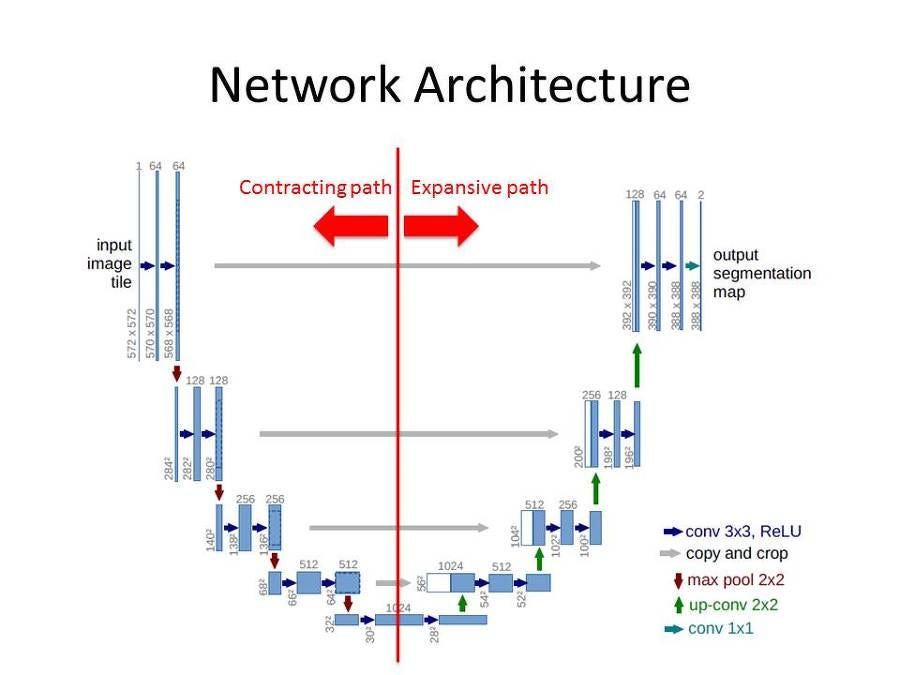
\includegraphics[width=0.7\linewidth]{3_Chapters//3_Chapter_Methodology//Figures/Unet.jpg}
	\caption{illustrates the \gls{U-Net} architecture, which transforms a grayscale input image into a smaller binary segmentation map using a contracting-expansive path with skip connections and no padding, progressively reducing spatial dimensions while increasing feature depth.}
	\label{fig:Unet}
\end{figure}

\subsubsection*{\gls{N2N}}
Lehtinen et al. \cite{pmlr-v80-lehtinen18a} developed \gls{N2N}  to address the challenge of requiring clean and noisy image pairs during the model training phase. \gls{N2N} makes use of two noisy images each with an independent noise distribution to learn the underlying signal from these noise-corrupted data points. Studies have shown \gls{N2N} achieving comparable performance to models trained with clean images. For instance, Lehtinen et al. \cite{pmlr-v80-lehtinen18a} trained the \gls{N2N} for 300 epochs with noisy targets and achieved an average \gls{PSNR} of 31.10 dB on the validation set, while training with clean targets reached 31.14 dB, comparable to previous work by Wang et al. \cite{wang2016accelerating} and Lee et al. \cite{7950457}. Additionally, \gls{N2N} can generalise across various types of noise distributions \cite{pmlr-v80-lehtinen18a}. The use of noisy image pairs during training and adapting to various noise types makes \gls{N2N} a highly suitable model for denoising LODOX\textsuperscript{\textregistered} Statscan\textsuperscript{\textregistered} images where noise is prevalent and acquiring images is impossible.

\textbf{Theory}\\
N2N improves on the traditional CNN model by eliminating the dependency on input data on the equation \ref{eq:emprisk} and using a trivial $f_{\theta}$ that outputs a learned scalar. This task reduces to a loss function, which can be viewed as an \gls{ML} estimation by interpreting the loss function as the negative log-likelihood as shown in equation \ref{eq:min_expectation} below:
\begin{equation}
	\arg\min_{\theta} \mathbb{E}_{x} \left\{ \mathbb{E}_{y|x} \left[ L(f_{\theta}(x), y) \right] \right\}
	\label{eq:min_expectation}
\end{equation}
From the above, it is deduced that the network can solve the point estimation problem separately for each input sample. Thus \gls{N2N} works on the principle that the property of L2 minimisation that on expectation, the estimate remains unchanged when the targets are replaced with random numbers whose expectations match the targets. Consequently, the loss function holds under these conditions, and the optimal network parameters $\theta$ of Equation \ref{eq:min_expectation} also remain unchanged, if input-conditioned target distributions $p(y|x)$  are replaced with arbitrary distributions that have the same conditional expected values.  As a consequence and  factoring in the use of corrupted inputs the empirical minimisation task reduces to equation \ref{eq:min_loss} below:
\begin{equation}
	\arg\min_{\theta} \sum_{i} L\left( f_{\theta}(\hat{x}_i), \hat{y}_i \right)
	\label{eq:min_loss}
\end{equation}

With inputs being drawn from a corrupted distribution that is conditioned on the underlying, unobserved clean target $y_i$ such that  $E\{\hat{y}_i|\hat{x}_i\} = y_i$, given an infinite data, the solution is the same as that of equation \ref{eq:emprisk} of traditional \gls{CNN}.

\gls{N2N}  starts with  a pair of  noisy image pairs  ($x^j$, $x^{j'}$), where

\begin{equation}
	x^j = s^j + n^j \quad \text{and} \quad x^{j'} = s^{j'} + n^{j'}
	\label{eq:noisemodel}
\end{equation}

The two training images are identical up to their noise components $n^j, n^{j'}$. Applying patch-based approach the training data is then viewed as pairs ${\mathbf{x}}_{{\text{RF}}(i)}^j, {{\mathbf{x}}_i}^{'j}$, consisting of a noisy input patch ${\mathbf{x}}_{{\text{RF}}(i)}^j$, extracted from $x^j$, and a noisy target, taken from $x^{'j}$ at the position i. Similarly, to traditional \gls{CNN} training, parameters are tuned to minimise the loss in equation \ref{eq:loss}, however, the only difference is that a noisy target is being used instead of ground truth data $y_i$. 

\textbf{Architecture} \\
\gls{N2N} architecture is a modified \gls{U-Net} architecture consisting of the following three key parts:
\begin{enumerate}
	\item \textbf{Contraction Part:} The contraction part consists of multiple Conv2D layers with 3x3 filters, typically using 64 filters to capture features from the input image. Optional dropout layers can be included to prevent overfitting by randomly zeroing a fraction of input units during training. Max-pooling layers with 2x2 filters are used to down-sample the feature maps, reducing spatial dimensions while retaining important features.
	\item \textbf{Bottleneck Part:} In the bottleneck, two Conv2D layers with 3x3 filters further process the down-sampled feature maps. Optional dropout layers can be applied to prevent overfitting. Up-sampling with 2x2 layers increases the spatial dimensions, preparing the feature maps for the expansion phase.
	\item \textbf{Expansion Part:} The expansion part includes Conv2D layers with 3x3 filters to refine the up-sampled feature maps and reconstruct the denoised image. Optional dropout layers help improve generalisation. 2x2 up-sampling layers restore the spatial dimensions of the feature maps to match the original input size.
\end{enumerate}
The architecture of a sample \gls{N2N} is visualised in Figure \ref{fig:N2Narch} below:

\begin{figure}[h!]
	\centering
	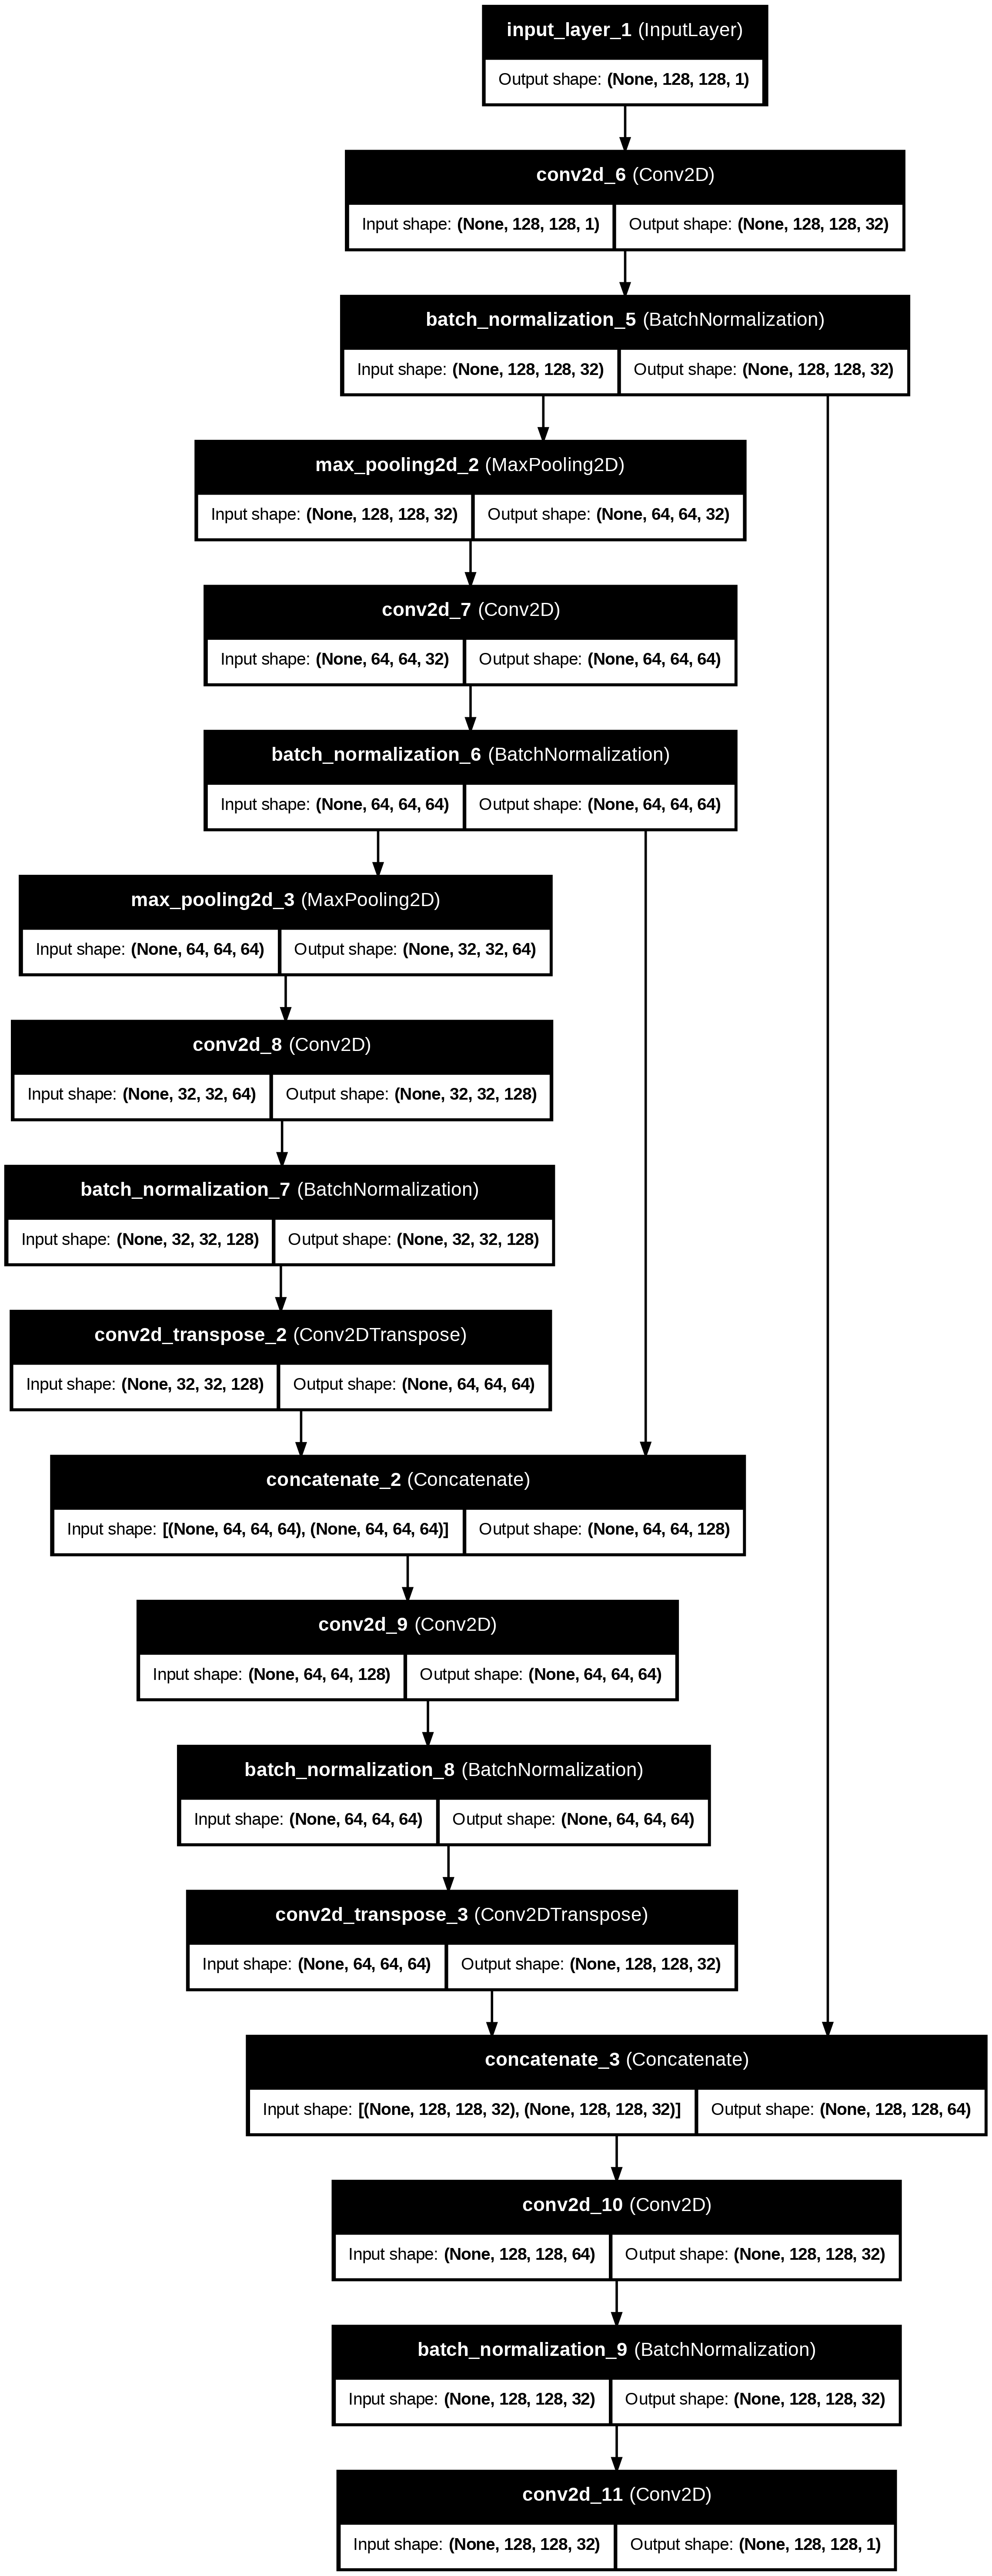
\includegraphics[width=0.25\linewidth]{3_Chapters//3_Chapter_Methodology//Figures/noise2noise_model.png}
	\caption{\gls{N2N} architecture}
	\label{fig:N2Narch}
\end{figure}

\subsubsection*{\gls{N2V}}
Krull et al. \cite{8954066} developed \gls{N2V} to eliminate the need for paired noisy images during the training phase. \gls{N2V} uses single noisy images to train the network to predict the values of randomly masked pixels, encouraging the model to learn spatial relationships in the data. This makes \gls{N2V} highly adaptable to various noise types as minimal assumptions about the underlying noise distribution are made. Krull et al. \cite{8954066}  demonstrated \gls{N2V} applicability to various imaging modalities by running experiments on photography, fluorescence microscopy, and cryo-Transmission Electron Microscopy. They concluded that as long as the assumptions of predictable signal and pixel-wise independent noise are met, \gls{N2V} performance is comparable to traditional and \gls{N2N}-trained models \cite{8954066}. Since \gls{N2V} does not require clean images or paired noisy images, it is a highly scalable solution, well-suited for LODOX\textsuperscript{\textregistered} Statscan\textsuperscript{\textregistered} images.


\textbf{Theory} \\
\gls{N2V} is an extension of \gls{N2N} in that it proposes that the two patches be extracted from a single image instead of two.  It is based on the principle that upon extraction of a patch, the centre pixel can be masked and used as the target, allowing the network to learn to map the value at the centre of the input patch directly to the output. 

To achieve this \gls{N2V} has a set of assumptions:

\begin{enumerate}
	\item Image generation is seen as ${\mathbf{x}} = {\mathbf{s}}+ {\mathbf{n}}$ as a draw from the joint distribution $p({\mathbf{s}},{\mathbf{n}}) = p({\mathbf{s}})p({\mathbf{n}}|{\mathbf{s}})$
	\item $p({\mathbf{s}})$ is assumed to be an arbitrary distribution satisfying $p({{\mathbf{s}}_i}|{{\mathbf{s}}_j}) \ne p({{\mathbf{s}}_i})$ for two pixels i and j within a certain radius of each other, with pixel ${{\mathbf{s}}_i}$ of the signal not statistically independent. \label{it:second}
	\item With respect to ${\mathbf{n}}$ a conditional distribution of the following form is assumed: $p({\mathbf{n}}|{\mathbf{s}}) = \prod\limits_i {p({{\mathbf{n}}_i}{{\mathbf{s}}_i})} $, indicating pixels values of the noise are conditionally independent given the signal.
	\item Noise is assumed to be zero-mean i.e $\mathbb{E}[{{\mathbf{n}}_i}] = 0$ leading to $\mathbb{E}[{{\mathbf{x}}_i}] = {{\mathbf{s}}_i}$ \label{it:fourth}
\end{enumerate}

Based on the above assumptions, it can be deduced that acquiring multiple images with the same underlying signal but different noise realisations, and then averaging them, will converge toward the true signal.

\gls{N2V} uses a special receptive field with a blind spot at its centre, as shown in Figure \ref{fig:blind} below; thus, \gls{CNN} prediction ${{\mathbf{\hat s}}_i}$ for a pixel is affected by all input pixels in a square neighbourhood except for the input pixel ${{\mathbf{x}}_i}$ at its very location. This leads to less information than a traditional \gls{CNN}; however, this is the advantage of the blindspot network i.e. its inability to learn identities. This is done by a masking scheme that replaces the value in the centre of each input patch with a randomly selected value from the surrounding area.

\begin{figure}[h!]
	\centering
	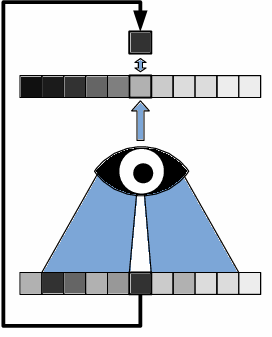
\includegraphics[width=0.3\linewidth]{3_Chapters//3_Chapter_Methodology//Figures/blindspot.png}
	\caption{Blind-spot network showing the receptive field of a pixel, excluding the pixel itself.}
	\label{fig:blind}
\end{figure}

The noise is assumed to be pixel-wise independent; thus, neighbouring pixels carry no information about the pixel, and therefore, it is impossible to produce an estimate that is better than a priori expected value(see \ref{it:fourth}). However, this is countered by the signal being assumed to contain statistical dependencies (see \ref{it:second}). As a result, the network can still estimate the signal ${{\mathbf{s}}_i}$ of a pixel by looking at its surroundings.  Consequently, the blind network allows extraction of input patch and target value from the same noisy image. Thus the empirical risk becomes:

\begin{equation}
	\mathop {\arg \min }\limits_\theta \sum\limits_j {\sum\limits_i {L\left( {f({\mathbf{\tilde x}}_{{\text{RF}}(i)}^j;\theta ),{\mathbf{x}}_i^j} \right)} } 
	\label{eq:minn2v}
\end{equation}

The target ${\mathbf{x}}_i^j$ is equivalent to \gls{N2N}'s ${\mathbf{x}}_i^{‘j}$ which is extracted from the second image. The two target values ${\mathbf{x}}_i^j$ and ${{\mathbf{x}}_i^{‘j}}$ have an equal signal ${{\mathbf{s}}_i^j}$with noise components being two independent samples from the same distribution $p({{\mathbf{n}}_i}|{{\mathbf{s}}_j})$. This, in principle, shows that using a blindspot network, an individual noisy image can be used to train the model. 

\textbf{Architecture}\\
\gls{N2V} is  based on a modified \gls{U-Net} architecture and consists of three main sections:

\begin{enumerate}
	\item \textbf{Contraction Part}: Multiple Conv2D layers with 3x3 filters (typically 64 filters each) capture features from the input image. Optional dropout layers prevent overfitting, and 2x2 max-pooling layers down-sample the feature maps, reducing spatial dimensions while retaining important features.
	\item \textbf{Bottleneck Part}: Two Conv2D layers with 3x3 filters further process the down-sampled feature maps. Optional dropout layers are included, and 2x2 up-sampling layers increase the spatial dimensions of the feature maps, preparing them for the expansion part.
	\item \textbf{Expansion Part}: Multiple Conv2D layers with 3x3 filters refine the up-sampled feature maps and reconstruct the denoised image. Optional dropout layers enhance generalisation, and 2x2 up-sampling layers restore the feature maps to the original input size. 
\end{enumerate}
A visual representation of the architecture is shown in Figure \ref{fig:N2Varch} below:
\begin{figure}[h!]
	\centering
	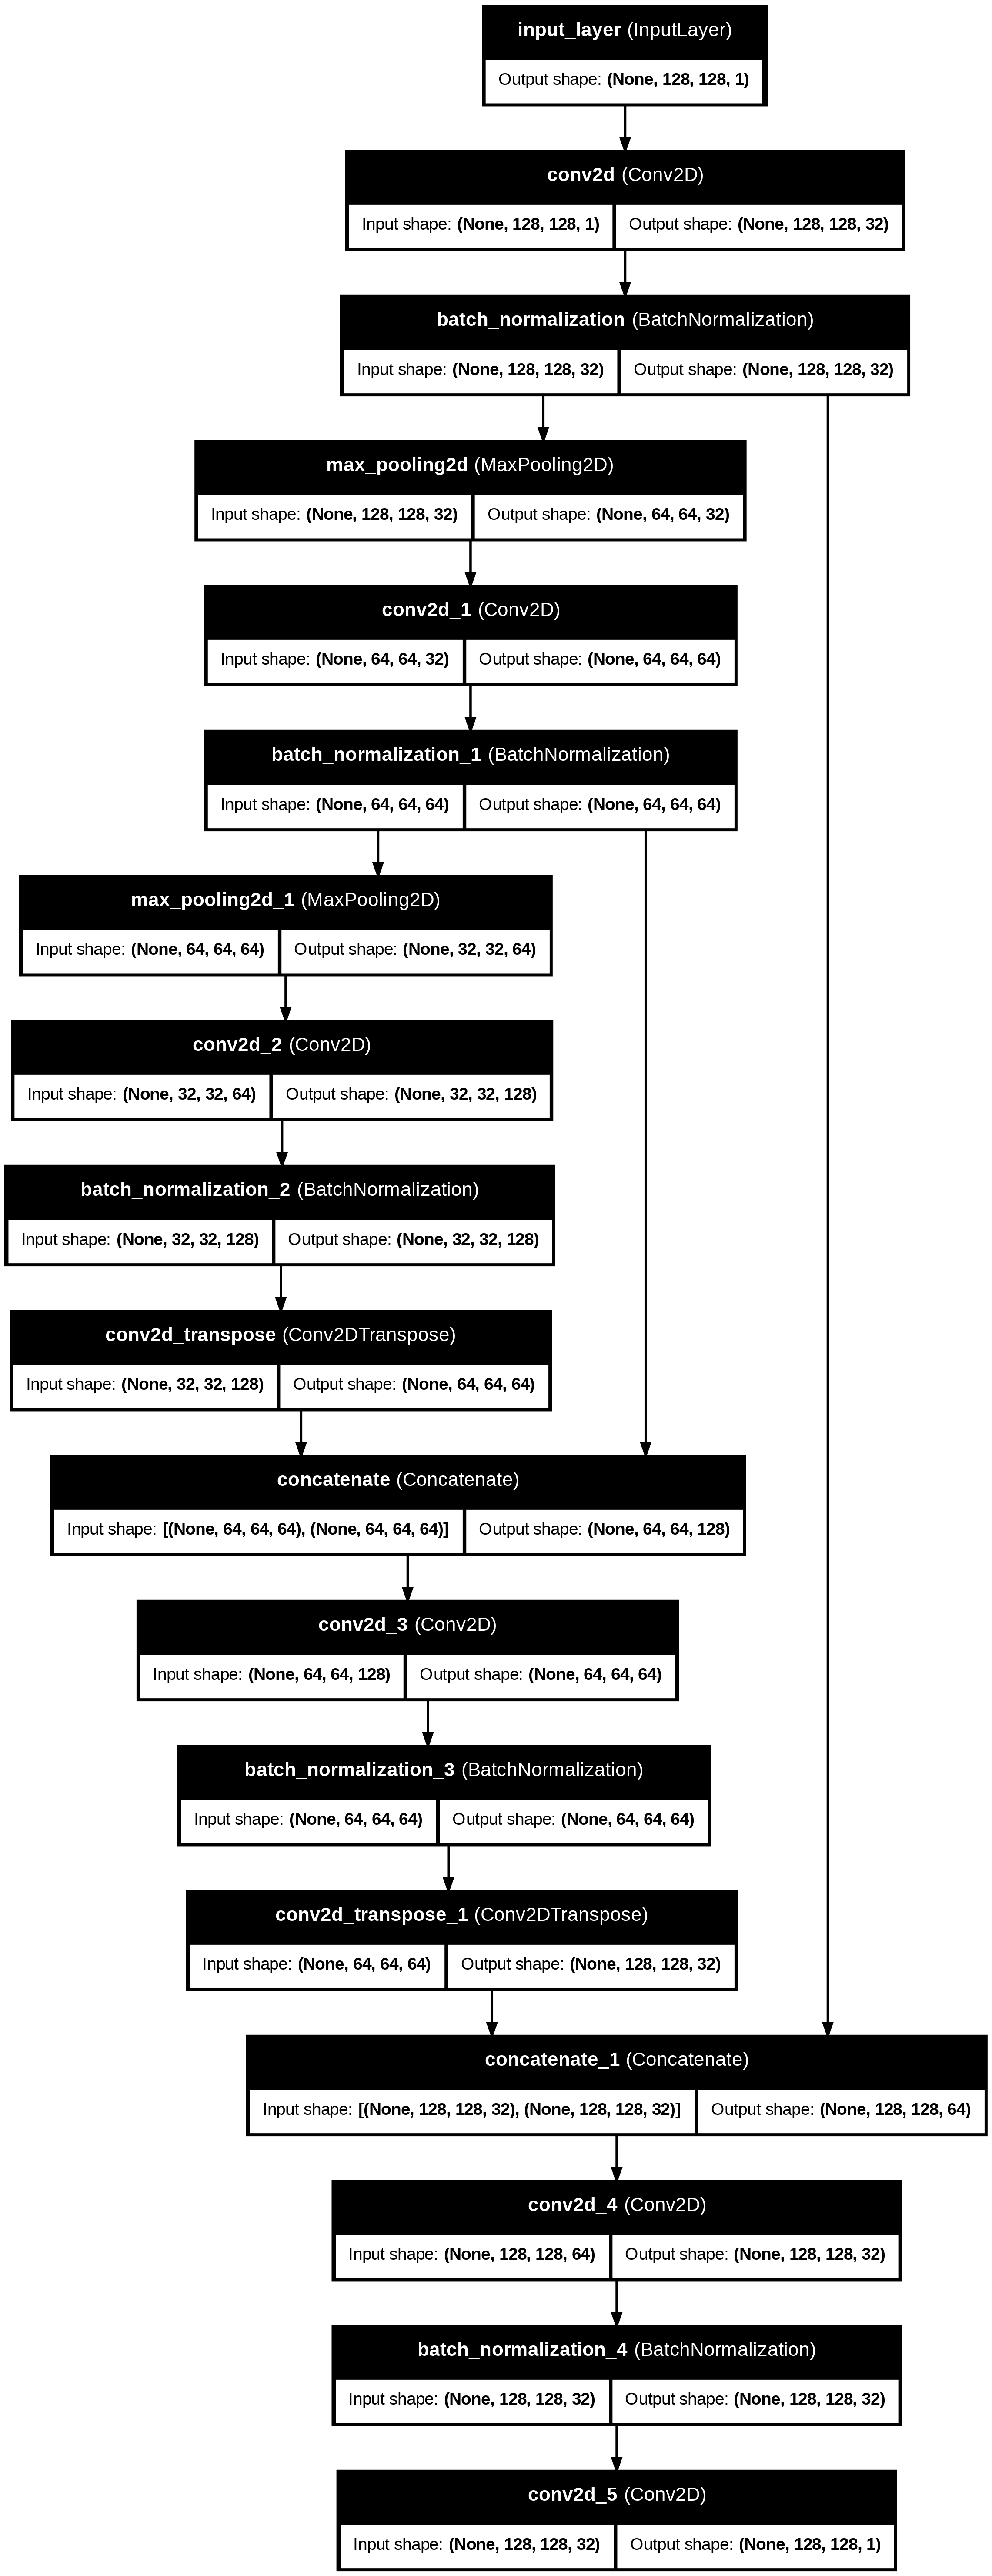
\includegraphics[width=0.25\linewidth]{3_Chapters//3_Chapter_Methodology//Figures/noise2void_model.png}
	\caption{\gls{N2V} architecture}
	\label{fig:N2Varch}
\end{figure}


\newpage
Both \gls{N2N} and \gls{N2V} are promising models for medical image denoising due to their unsupervised nature, effectively addressing the challenges of acquiring clean training data in a clinical context like Lodox imaging. Other attempts to denoise X-ray images primarily using supervised learning are discussed below.

Supervised models struggle to denoise images such as LODOX\textsuperscript{\textregistered} Statscan\textsuperscript{\textregistered} as no noiseless images are available to train the models. Zhang et al.'s \gls{DnCNN} model \cite{7839189}, though effective against traditional noise, struggles with Poisson noise common in low-dose imaging like LODOX\textsuperscript{\textregistered} Statscan\textsuperscript{\textregistered}. Hariharan's model-based approach \cite{hariharan_learning-based_2019} demonstrates strong results with simulated data, but its reliance on simulations limits real-world clinical applicability. Nadkarni et al.'s 2D \gls{U-Net} \gls{CNN} \cite{huber_dedicated_2022} and Chang et al.'s \gls{PKAID-Net} \cite{chang_improved_2024}, deliver high-quality denoising but similarly rely on supervised learning and complex iterative processes, which may hinder their effectiveness in LODOX\textsuperscript{\textregistered} Statscan\textsuperscript{\textregistered} settings where acquiring clean reference images is impractical. While these models are powerful, their supervised nature and dependency on high-quality training data pose challenges for effectively denoising LODOX\textsuperscript{\textregistered} Statscan\textsuperscript{\textregistered} images. 


\section{Conclusion}
%Will still need to be redone in a better way just a placeholder
The literature review provided a comprehensive analysis of classical and modern denoising techniques, mainly focusing on their applicability to low-dose systems such as the LODOX\textsuperscript{\textregistered} Statscan\textsuperscript{\textregistered} systems. 

The review began with a brief overview of X-ray imaging fundamentals, including X-ray production, attenuation, and detection and their significance to image quality. This was followed by an analysis of noise types in X-ray images. It was highlighted that the predominant noise degrading X-ray images is Poisson noise, and various Posison denoising methods were looked into. A plethora of classical \gls{DSP} filters was looked into, highlighting their limitations in handling photon-limited images. Despite some variations of wavelet and \gls{NLM} filters showing promise, they often fell short of effectively reducing Poisson noise without compromising image quality. The review then transitions to hybrid filters, particularly the \gls{BM3D}. \gls{BM3D} demonstrates significant improvement over classical filters but still faces challenges in denoising noise-heavy images such as LODOX\textsuperscript{\textregistered} Statscan\textsuperscript{\textregistered} images. This underscored the need for adaptable denoising methods to learn different noise patterns.

\gls{ML} methods like \gls{N2N} and \gls{N2V} offer significant potential due to their ability to operate without clean training data. This is critical for LODOX\textsuperscript{\textregistered} Statscan\textsuperscript{\textregistered} as it is impossible to obtain ground truth data. However, in most of the literature, the testing was mostly done on \gls{MRI}, \gls{CT} and microscopy images, with limited application to low-dose X-ray systems like the LODOX\textsuperscript{\textregistered} Statscan\textsuperscript{\textregistered}. While \gls{N2N} and \gls{N2V} have shown adaptability across various noise types in other imaging domains, applying these models to the LODOX\textsuperscript{\textregistered} Statscan\textsuperscript{\textregistered} system presents both a challenge and an opportunity for further research. This project aims to bridge this gap by adapting and enhancing \gls{N2N} and \gls{N2V} models specifically for LODOX\textsuperscript{\textregistered} Statscan\textsuperscript{\textregistered} images, documenting the results and challenges encountered in this process. This approach addresses the current limitations in the literature and contributes to the development of more effective denoising techniques for low-dose X-ray imaging.
